\chapter{Results} \label{results}

\section{Theoretical Maximum}
As has been established, the maximum performance scales with the available memory bandwidth of the system, and not with the amount of processes used. For SpMV, a total of 6 bytes are read per FLOP, which means that the theoretical maximum is given by \ref{eq:theoretical_max}. This is under the assumption that all resources on the system is dedicated to the SpMV operation, which is not the case in reality. At most, somewhere in the neighbourhood of 80\% of the systems resources can be expected to be utilized.

\begin{equation}
\text{Maximum Theoretical Performance} = \frac{\text{Memory bandwidth}}{6}
\label{eq:theoretical_max}
\end{equation}


\section{Matrices}
For the results presented in the following sections, the matrices shown in Figure \ref{fig:matricesused} were selected as they are in general well-structure and symmetrical. 

\begin{figure}[H]
  \centering
  \captionsetup[sub]{font=tiny, textfont=tiny}
  \setlength{\tabcolsep}{4pt} % adjust horizontal padding between columns
  \begin{tabular}{cccc}
      \subcaptionbox{\tiny{bone010}\label{fig:bone010}}{%
      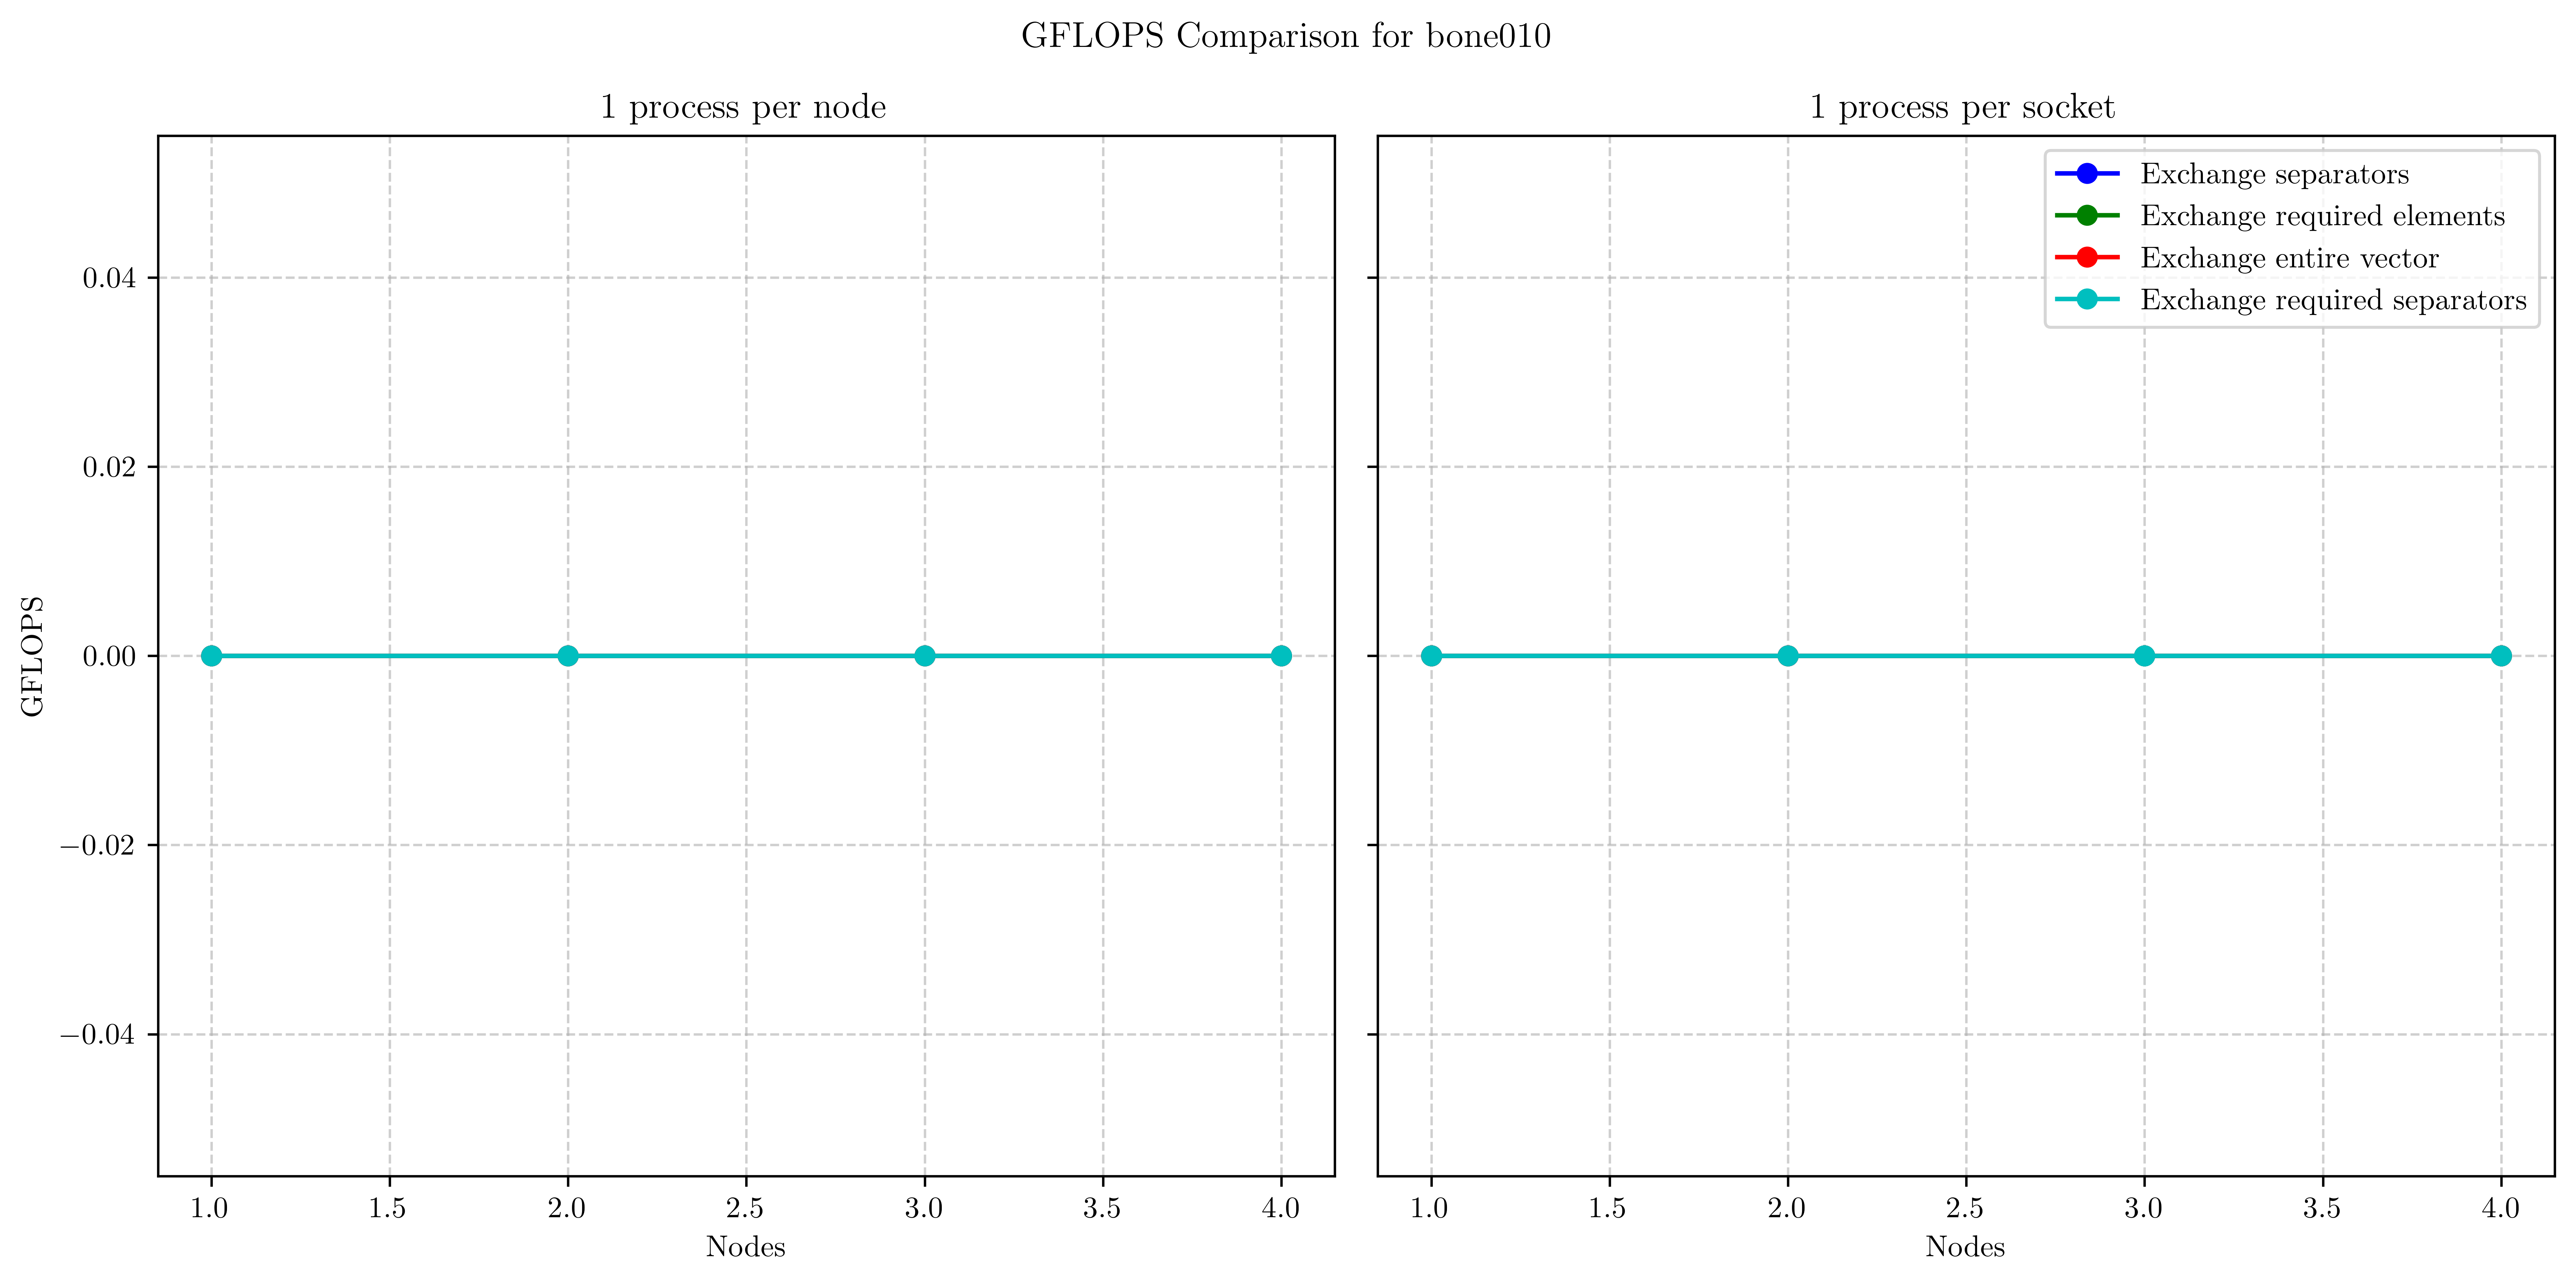
\includegraphics[width=0.23\textwidth]{bone010.png}%
    } &
    \subcaptionbox{\tiny{af\_shell10}\label{fig:af_shell10}}{%
      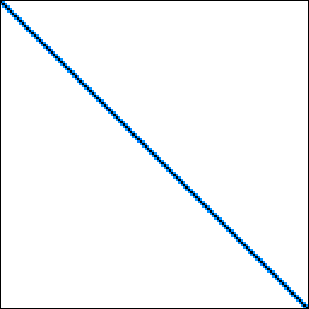
\includegraphics[width=0.23\textwidth]{af_shell10.png}%
    } &
    \subcaptionbox{\tiny{Serena}\label{fig:Serena}}{%
      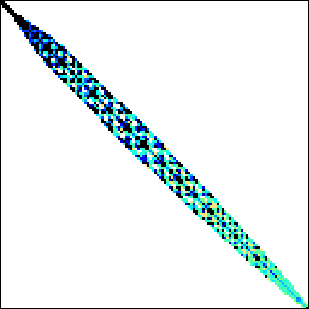
\includegraphics[width=0.23\textwidth]{Serena.png}%
    } &
    \subcaptionbox{\tiny{Long\_Coup\_dt0}\label{fig:Long_Coup_dt0}}{%
      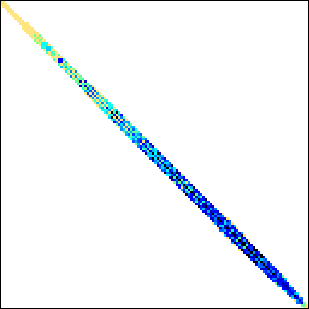
\includegraphics[width=0.23\textwidth]{Long_Coup_dt0.png}%
    } \\[6pt] % a little extra vertical gap
    \subcaptionbox{\tiny{dielFilterV3real}\label{fig:dielFilterV3real}}{%
      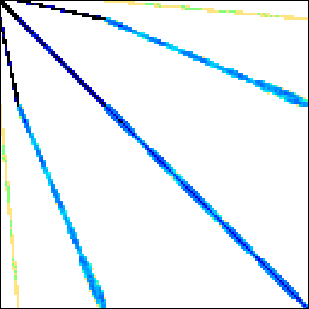
\includegraphics[width=0.23\textwidth]{dielFilterV3real.png}%
    } &
    \subcaptionbox{\tiny{Cube\_Coup\_dt0}\label{fig:Cube_Coup_dt0_1}}{%
      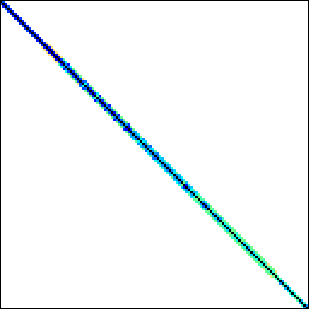
\includegraphics[width=0.23\textwidth]{Cube_Coup_dt0.png}%
    } &
    \subcaptionbox{\tiny{Bump\_2911}\label{fig:Bump_2911}}{%
      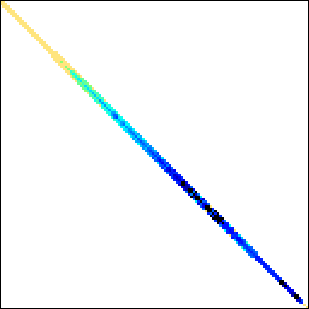
\includegraphics[width=0.23\textwidth]{Bump_2911.png}%
    } &
    \subcaptionbox{\tiny{nlpkkt200}\label{fig:nlpkkt200}}{%
      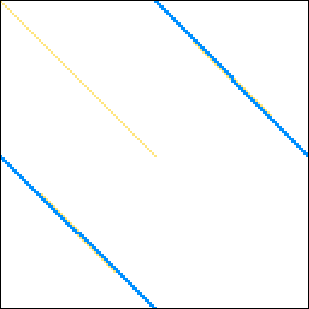
\includegraphics[width=0.23\textwidth]{nlpkkt200.png}%
    }
  \end{tabular}
  \caption{Matrices used to generate results.}
  \label{fig:matricesused}
\end{figure}

\begin{table}[H]
\begin{center}
\begin{tabular}[c]{|l|l|}
\hline
\textbf{Name}&\textbf{Purpose}  \\
\hline
bone010&Trabecular Bone Micro-Finite Element Model\\
\hline
af\_shell1&Sheet metal forming matrix\\
\hline
Serena&Gas reservoir simulation for \(CO_{2}\) sequestration\\
\hline
Long\_Coup\_dt0&3D coupled consolidation problem (geological formation)\\
\hline
dielFilterV3real&High-order vector finite element method in EM\\
\hline
Cube\_Coup\_dt0&3D coupled consolidation problem (3D cube)\\
\hline
Bump\_2911&3D geomechanical reservoir simulation\\
\hline
nlpkkt200&Symmetric indefinite KKT matrix\\
\hline
\end{tabular}
\end{center}
\end{table}


\section{Overview of Experiments}
Experiments have been ran on several systems available on Simulas eX\(^{3}\) machine. The systems the experiments have been ran on are \defq, \romeq\phantom{a}and \fpgaq.
\medskip

For each experiment, every matrix has been put through 100 iterations of SpMV, and every communication strategy has been tested on different configurations. For the single node experiments, each communication strategy has been ran with the number of MPI ranks being doubled until every available physical core on the chip is assigned one MPI rank. For multi node experiments on single socketed nodes, one MPI rank is assigned to each rank, and shared memory parallelization has been used within each node. On dual socketed nodes, experiments placing one MPI rank per node and placing one MPI rank per socket have been ran. All programs have been compiled with \texttt{-march=native} and \texttt{-O3} compilation flags.

% \begin{table}[H]
%     \begin{center}
%         \begin{tabular}[c]{|p{3cm}|p{3cm}|p{3cm}|p{3cm}|}
%             \hline
%             &\textbf{\defq}&\textbf{\fpgaq}&\textbf{\romeq}  \\
%             \hline
%             No. of sockets&2&2&1  \\
%             \hline
%             No. of physical cores per socket&32&24&16  \\
%             \hline
%             No. of nodes&4&4&8  \\
%             \hline
%             Tested single node performance&Yes&No&No  \\
%             \hline
%             Single Node Ranks&\(1,2,4,8,16,32,64\)&N/A&N/A  \\
%             \hline
%         \end{tabular}
%     \end{center}
%     \caption{Configurations used on experiments}
% \end{table}

In the following presentation of the results, \ref{tab:commstratdesc} gives an overview of what the different strategies will be referred to, both when analyzing the results, and in the legends of the figures.

\begin{table}[H]
    \begin{center}
        \begin{tabular}[c]{|p{3cm}|p{5cm}|}
            \hline
             \textbf{Strategy name}& \textbf{Strategy Description}  \\
            \hline
             Strategy A&Exchanges entire local vector.  \\
            \hline
             Strategy B&Exchanges entire separator.  \\
            \hline
             Strategy C&Exchanges required separator.  \\
            \hline
             Strategy D&Exchanges required separator elements  \\
            \hline
             Strategy E&Exchanges required separator elements, memory scalable  \\
            \hline
        \end{tabular}
    \end{center}
    \label{tab:commstratdesc}
\end{table}

\section{\defq - Single Node Performance}
The results in this section illustrates the performance of the communication strategies when performed on a single node containing two \defq\phantom{a}chips.  
\begin{figure}[H]
    \centering
    \incfig[1]{gflops\_2x4\_single\_defq}
    \caption{Sustained performance (GFLOPS) over 100 iterations of SpMV on a single node equipped with dual-socket \defq{} processors.}
    \label{fig:gflopsdefqsingle}
\end{figure}
Figure \ref{fig:gflopsdefqsingle} presents the achieved GFLOPS for each communication strategy. The performance trends largely align with expectations: each successive strategy generally exhibits improved performance over its predecessor. However, an exception arises with strategy E, which consistently underperforms relative to strategy D.
\medskip

As discussed in section \ref{sec:memscal}, strategy E reorders the local vector and separators. The effect this reordering has on well ordered matrices is that it can reduce cache reuse. This has not been measured directly, but it is the most likely culprit to the discrepancy between the results of strategy D and E.

% As detailed in Algorithm \ref{alg:reqsepexchange}, strategy E incurs a significant overhead due to its requirement to pack and unpack every individual element exchanged across separator boundaries. This repeated packing and unpacking operation introduces substantial computational and memory overhead, which offsets the potential benefits of the strategy and explains its inferior performance. It is however important to keep in mind that the goal of strategy E is not necessarily to achieve the absolute highest possible GFLOPS performance, but rather to ensure that it is scalable to large matrices, and is able to run on architectures that have lower local memory.
 
\begin{figure}[H]
    \centering
    \incfig[1]{t\_2x4\_single\_defq}
    \caption{Total execution time of each communication strategy on a single node equipped with dual-socket \defq{} processors.}
    \label{fig:tdefqsingle}
\end{figure}

Figure \ref{fig:tdefqsingle} presents the total execution time for each communication strategy. It is closely related to Figure \ref{fig:gflopsdefqsingle}, as computing the GFLOPS number is given by the total number of flops performed divided by the total execution time.

% \begin{equation}
%     \label{eq:gflops}
%     \text{GFLOPS} = \frac{\text{No. of flops performed}}{\text{Total execution time}}
% \end{equation}

\begin{figure}[H]
    \centering
    \incfig[1]{tcomm\_2x4\_single\_defq}
    % \caption{Communication time component of each strategy on a single node using the \defq{} chip.}
    \caption{Communication time per iteraton of SpMV on a single node equipped with dual-socket \defq{} processors.}
    \label{fig:tcommdefqsingle}
\end{figure}

Figure \ref{fig:tcommdefqsingle} present the time spent communicating the data data-dependencies between MPI ranks for each iteration of SpMV. The results clearly illustrate the performance benefits of optimizing communication in distributed single node SpMV. Strategy A acts as a baseline, by naively communicating the entire vector. Each successive communication strategy implements measures to reduce the communication volume, and it can be seen that this does indeed result in lower communication times. Strategy B limited communication to communicating only separators, Strategy C narrowed this to only communicating the separators to the rank that need them. Finally, strategy D and E further reduces the communication volume by only communicating necessary separator elements. This progresion confirms the role communication strategies play in reducing the bottleneck that the data-dependencies between nodes induce. The results emphasize that careful attention to communication minimization yields improvements communication time, and by extension in performance for memory-bound operations like SpMV.

\begin{figure}[H]
    \centering
    \incfig[1]{tcomp\_2x4\_single\_defq}
    \caption{Computation time per iteraton of SpMV on a single node equipped with dual-socket \defq{} processors.}
    \label{fig:tcompdefqsingle}
\end{figure}

\begin{figure}[H]
    \centering
    \incfig{commload\_2x4\_single\_defq}
    \caption{Fraction of the size of the global \(x\) vector communicated per SpMV iteration.}
    \label{fig:commloaddefqsingle}
\end{figure}
Figure \ref{fig:commloaddefqsingle} shows the fraction of the input vector \(x\) communicated per SpMV iteration across various matrices and ranks for different communication strategies. This figure provides an important quantitative counterpart to the timing data: it confirms that strategies which yielded lower communication time also effectively minimized the volume of communicated data. The results presented in this figure only show the communication volume for strategies B-D. Strategy A have been left out as the fraction of \(x\) communicated in each iteration is 1 no matter how many ranks are used. Strategy E has been left out as the communication volume for this strategy is the same as strategy D.
\medskip

Notably, when comparing strategy B and C, the rank with the maximum communication volume in strategy C is usually equal to, or lower than the average communication volume of strategy B.



\medskip


% \inputdefqsingle.tex}
\section{(Rome16q) \romeq}
\begin{figure}[H]
    \centering
    \incfig[1]{gflops\_2x4\_multi\_rome16q}
    \caption{Sustained GFLOPS performance of SpMV over 100 iterations on 1–8 nodes (one MPI rank per node) using single-socket \romeq{} processors.}
    \label{fig:gflopsromemulti}
\end{figure}

Figure \ref{fig:gflopsromemulti} presents the achieved GFLOPS across up to eight single-socket nodes using the \romeq{} processor. These results offer a more fine-grained perspective on the performance of various communication strategies, particularly when employing a non-power-of-two number of MPI ranks. In contrast to the single node experiments discussed in Section \ref{sec:singlenode}, where the number of ranks were limited to powers of two, this linear range of nodes shows how the communication strategies behave under less ideal conditions.
\medskip



% The number of ranks for the single node results seen in Section \ref{sec:singlenode} were restricted to be powers of two, and as with everything in the computing world - powers of two tends to behave nicely.

%  In contrast to the single-node experiments discussed in Section \ref{sec:singlenode}, which were limited to powers of two, this broader range allows us to observe behaviors under less idealized conditions. As is often the case in computing, configurations based on powers of two tend to exhibit more regular and favorable performance characteristics.

% Strategy A exhibits a sawtooth-like pattern depending on whether the number of nodes is even or odd. This is due to a quirk of how MPI decides to work (see \cite{10064025}).

\begin{figure}[H]
    \centering
    \incfig[1]{t\_2x4\_multi\_rome16q}
    \caption{Total execution time for 100 iterations of SpMV on 1–8 nodes (one MPI rank per node) using single-socket \romeq{} processors.}
    \label{fig:tromemulti}
\end{figure}

\begin{figure}[H]
    \centering
    \incfig{tcomp\_2x4\_multi\_rome16q}
    \caption{Computation time per iteration of SpMV on 1–8 nodes (one MPI rank per node) using single-socket \romeq{} processors.}
    \label{fig:tcomp2x4multirome16q}
\end{figure}

\begin{figure}[H]
    \centering
    \incfig[1]{tcomm\_2x4\_multi\_rome16q}
    \caption{Communication time per iteration of SpMV on 1–8 nodes (one MPI rank per node) using single-socket \romeq{} processors.}
    \label{fig:tcommromemulti}
\end{figure}

The results in Figure \ref{fig:tcommromemulti} present the communication time per iteration of SpMV on up to eight \romeq{} nodes. Notably, Strategy A exhibits a sawtooth-like pattern, depending on whether or not the number of nodes used is even or odd. Such irregularities is can be explained by the underlying communication algorithms MPI decides to employ when using \texttt{MPI\_Allgatherv}. MPI decides on some internal algorithm to use in collective communication routines, depending on the number of ranks involved in the operation and the size of the messages amongst other factors. The exact algorithm MPI uses internally for these results is unknown, and outside the scope of this thesis, but it is the most probable reason that this sawtooth pattern is observed, this is also backed up by the fact that the results in Figure \ref{fig:tcomp2x4multirome16q}, which illustrate the computation time for each strategy, don't exhibit this behaviour.

\begin{figure}[H]
    \centering
    \incfig[1]{commload\_2x4\_multi\_rome16q}
    \caption{Fraction of the global \(x\) vector communicated per iteration of SpMV on 1–8 nodes (one MPI rank per node) using single-socket \romeq{} processors.}
    \label{fig:commlaoadromemulti}
\end{figure}


\section{(defq) \defq}
\section{(defq multi) \defq}
\begin{figure}[H]
    \centering
    \incfig[1]{gflops\_2x4\_multi\_defq}
    \caption{multi Node - \defq}
    \label{fig:gflopsdefqmulti}
\end{figure}

\begin{figure}[H]
    \centering
    \incfig[1]{tcomm\_2x4\_multi\_defq}
    \caption{}
    \label{fig:tcommdefqmulti}
\end{figure}


\begin{figure}[H]
    \centering
    \incfig{commload\_2x4\_multi\_defq}
    \caption{}
    \label{}
\end{figure}

\subsection{2 proc per node}

\begin{figure}[H]
    \centering
    \incfig[1]{gflops\_2x4\_multi\_defqmpi}
    \caption{Multi Node - \defq}
    \label{fig:gflopsdefqmpimulti}
\end{figure}

\begin{figure}[H]
    \centering
    \incfig[1]{tcomm\_2x4\_multi\_defqmpi}
    \caption{}
    \label{fig:tcommdefqmpimulti}
\end{figure}


\begin{figure}[H]
    \centering
    \incfig{commload\_2x4\_multi\_defqmpi}
    \caption{}
    \label{}
\end{figure}





% eX3 - High-Performance Computing Reports
%
% Copyright (C) 2020 Simula Research Laboratory
% Authors: James D. Trotter <james@simula.no>
%
% Hardware

\begin{table}[ht]
  \centering
  \linespread{0.85}\renewcommand{\arraystretch}{1.2}
  \setlength{\tabcolsep}{2pt}    % a little padding between columns
  \footnotesize\sffamily
  %--------------------------------------------------------------------------------
  % use tabular* + \extracolsep{\fill} to force it to exactly \textwidth
  \begin{tabular*}{\textwidth}{@{\extracolsep{\fill}}
      l
      >{\raggedleft\arraybackslash}p{0.18\textwidth}
      >{\raggedleft\arraybackslash}p{0.18\textwidth}
      >{\raggedleft\arraybackslash}p{0.18\textwidth}
    @{}}
    \toprule
      & {\small FPGAQ}
      & {\small Rome}
      & {\small Defq} \\
    \midrule
    CPUs
      & \fpgaq{} 
      & \romeq{} 
      & \defq{} \\

    Instr.\ setu w
      & x86-64
      & x86-64
      & x86-64 \\

    Microarch.
      & Zen 3
      & Zen 2
      & Zen 1 \\

    Sockets
      & 2
      & 1
      & 2 \\

    Cores
      & $2\times24$
      & $1\times16$
      & $2\times32$ \\

    Freq.~[GHz]
      & $2.6$--$3.6$
      & $1.5$--$3.3$
      & $2.2$--$3.2$  \\

    \midrule
    L1I/core [KiB]
      & 64
      & 32
      & 64\\

    L1D/core [KiB]
      & 32
      & 32
      & 32 \\

    L2/core [KiB]
      & 512
      & 512
      & 512 \\

    L3/socket [MiB]
      & 128
      & 16
      & 128 \\

    Mem.\ channels
      & $2\times8$
      & $1\times8$
      & $2\times8$ \\

    Bandwidth [GB/s]
      & N/A
      & 204.8
      & N/A\\

    Triad [GB/s]
      & N/A
      & 90.9
      & N/A \\
    \bottomrule
  \end{tabular*}
  \caption{Hardware used in the experiments. STREAM Triad was run with the \texttt{-march=native} and \texttt{-O3} compilation flags.}
  \label{tab:hardware}
\end{table}



% \begin{table*}[thb]
%   \centering
%   \caption{\small Hardware used in our experiments. STREAM Triad \cite{mccalpin1995memory} was run with the \texttt{-march=native} and  \texttt{O3} compilation flags.}
%   \footnotesize
%   \setlength{\tabcolsep}{4pt}
%   \resizebox{\textwidth}{!}{
%   \begin{tabular}{lrrrrrr}
%     \toprule
%     Chip	&	{\scriptsize AMD Epyc}	&	{\scriptsize AMD Epyc}	&	{\scriptsize AMD Epyc}	&	{\scriptsize AMD Epyc}	&	{\scriptsize Intel Xeon}	&	{\scriptsize Intel Xeon}	\\
%     Model	&	{\scriptsize 7763}	&	{\scriptsize 7601}	&	{\scriptsize  7413}	&	{\scriptsize 7302P}	&	{\scriptsize Gold 6130}	&	{\scriptsize Platinum 8360Y}	\\
%     \midrule													
%     Instruction set	&	x86-64	&	x86-64	&	x86-64	&	x86-64	&	x86-64	&	x86-64	\\
%     Microarchitecture	&	Zen3	&	Zen	&	Zen3	&	Zen2	&	 Skylake (server) 	&	Ice Lake (server)  	\\
%     Cores/Threads	&	2 $\times$ 64/128	&	2 $\times$ 32/64	&	2 $\times$ 24/48	&	16/32	&	 2 $\times$ 32/64     	&	  2 $\times$ 36/72 	\\
%     Core frequency(GHz)	&	2.45 to 5.5	&	2.7 to 3.2	&	2.65 to 3.6	&	3.0 to 3.3	&	 1.9 to 3.6  	&	  1.8 to 3.6 	\\
%     L1I/L1D/L2 (KiB per core)	&	32/32/512	&	64/32/512	&	32/32/512	&	32/32/512	&	32/32/1024	&	 32/48/1280 	\\
%     L3 cache (MiB)	&	2 $\times$ 256 (8 $\times$ 32)	&	2 $\times$ 64 (8 $\times$ 8)	&	2 $\times$ 128 (4 $\times$ 32)	&
%                                                                                                                                                  128 (8 $\times$ 16)		&	2 $\times$ 22 	&	2 $\times$ 54	\\
%     Memory Channels	&	 2 $\times$ 8 	&	 2 $\times$ 8 	&	 2 $\times$ 8 	&	8	&	2 $\times$ 6	&	 2 $\times$ 8 	\\
%     Total Memory (GB)	&	2048	&	2048	&	512	&	256	&	384	&	2048	\\
%     Max.~bandwidth (GB/s)	&	381.4	&	340.8	&	381.4	&	190.7	&	238.4	&	381.4	\\
%     STREAM Triad (GB/s)	&	200.8	&	161.4	&	200.8	&	90.6	&	147.1	&	293.1	\\
%     \addlinespace
%     \bottomrule
    
%   \end{tabular}}
%   \label{tbl:hardware}
% \end{table*}
% %milan 8*32




    %  Chip & {\scriptsize AMD Epyc} & {\scriptsize Intel Xeon } & {\scriptsize AMD Epyc } & {\scriptsize Cavium ThunderX2} & {\scriptsize HiSilicon Kunpeng} \\
    %  Model & {\scriptsize 7302P} & {\scriptsize Gold 6130} & {\scriptsize 7601} & {\scriptsize  CN9980} & {\scriptsize 920-6428} \\ 
    % \midrule
    % Instruction set      & x86-64             & x86-64           & x86-64    & ARMv8.1  & ARMv8.2    \\
    % Microarchitecture    & Zen 2       & Skylake (server) & Zen      & 	Vulcan  & TaiShan v110      \\
    % Cores/Threads        & 16/32              & 2 $\times$ 32/64     & 2 $\times$ 32/64 &  2 $\times$ 32/128   &  2 $\times$ 64/64    \\
    % Core frequency (GHz)      & 3.0 to 3.3       & 1.9 to 3.6  & 2.7 to 3.2 &  2.0 to 2.5  &  2.8   \\
    % L1I/L1D/L2 (KiB per core)     & 32/32/512     & 32/32/1024    & 64/32/512   & 32/32/256 & 64/64/512  \\  
    % L3 cache (MiB per socket)  & 128 (8x16) 	  & 22 (16x1.375)   & 64	(8x8)  & 32	(32x1)  & 64	(64x1)  \\
    % Memory Channels        &  8 & 2 $\times$ 6  & 2 $\times$ 8 & 2 $\times$ 8 & 2 $\times$ 8  \\
    % Total Memory (GB)        & 256 & 384 & 2048 & 1024 & 1024  \\  
    % Max.~bandwidth (GB/s)      & 204.8       & 238.4        & 340.8  & 317.9   & 381.4   \\
    %       STREAM Triad  (GB/s)             & 90.6       & 147.1      & 161.4  &  173.3 &  193.5  \\
                         
    %                      \addlin


